\documentclass[../main.tex]{subfiles}

\begin{document}
	\section{Gradino}
	\begin{figure}[h!]
		\centering
		\begin{subfigure}{0.4\textwidth}
			\[
				1(t) = 
				\begin{cases}
					0 \quad t<0\\
					1 \quad t \geq 0
				\end{cases}
			\]
		\end{subfigure}
		\begin{subfigure}{0.4\textwidth}
			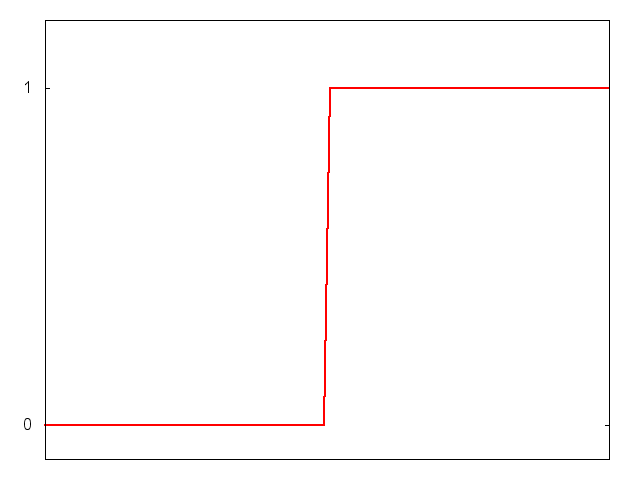
\includegraphics[width=5cm, height=3cm]{plot/funzioni_generalizzate/gradino}
		\end{subfigure}
	\end{figure}
	Presenta una discontinuità in $t=0$.
	%
	\section{Rampa}
	\begin{figure}[h!]
		\centering
		\begin{subfigure}{0.4\textwidth}
			\[
				ramp(t)=
				\begin{cases}
					0 \quad t<0\\
					t \quad t \geq 0			
				\end{cases}
			\]
		\end{subfigure}
		\begin{subfigure}{0.4\textwidth}
			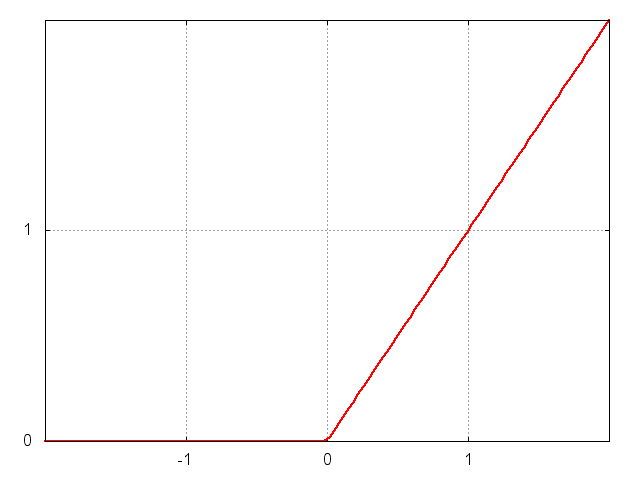
\includegraphics[width=5cm, height=3cm]{plot/funzioni_generalizzate/rampa}
		\end{subfigure}
	\end{figure}
	In $t=0$ e' continua, ma presenta una discontinuità di prima specie nella derivata.
	%
	\section{Parabola}
	\begin{figure}[h!]
		\centering
		\begin{subfigure}{0.4\textwidth}
			\[
				par(t)=
				\begin{cases}
					0 \quad &t<0\\
					\frac{t^2}{2} \quad &t\geq 0
				\end{cases}
			\]
		\end{subfigure}
		\begin{subfigure}{0.4\textwidth}
			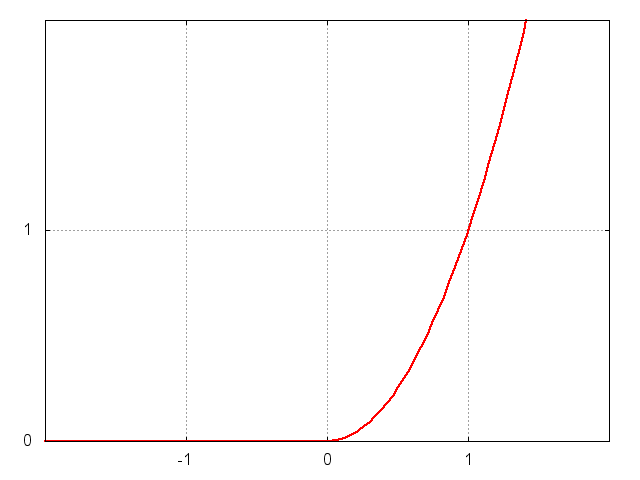
\includegraphics[width=5cm, height=3cm]{plot/funzioni_generalizzate/parabola}
		\end{subfigure}
	\end{figure}
	Risulta continua e con derivata continua anche in $t=0$.	
	%
	\section{Polinomio di grado n}
	\[
		pol(t)=
		\begin{cases}
			0 \quad &t<0\\
			\frac{t^n}{n} \quad &t\geq 0
		\end{cases}
	\]
	%
	\section{Derivate e integrali delle funzioni generalizzate}
	\begin{align*}
		&ramp(t) = \int_{- \infty}^{t} 1(\tau) \mathrm{d}\tau &&\der{}{t} ramp(t) = 1(t)\\
		&par(t) = \int_{- \infty}^{t} ramp(\tau) \mathrm{d} \tau &&\der{}{t} par(t) = ramp(t)	
	\end{align*}
	%
	\section{Impulso}
	Introduco la funzione $1_{\Delta}(t)$ definita come:
	%grafico della funzione e della derivata
	\[
		\int_{- \infty}^{t} \der{}{t}1_{\Delta}(t) \mathrm{d}\tau=
		\begin{cases}
			1 \quad t>\Delta\\
			0 \quad t<0
		\end{cases}
	\]
	Non consideriamo il caso in cui $0<t<\Delta$.\\
	\linebreak
	Definisco $\delta(t)$ la funzione $\der{}{t}1_{\Delta}(t)$ quando $\Delta \longrightarrow 0$. Valgono dunque le seguenti relazioni: 
	\begin{figure}[h!]
		\centering
		\begin{subfigure}{0.5\textwidth}
			\[
			\int_{-t}^{t} \delta(\tau) \mathrm{d}\tau =1 \quad \forall t>0, \qquad \der{}{t} 1(t) = \delta(t)
			\]
		\end{subfigure}
		\begin{subfigure}{0.4\textwidth}
			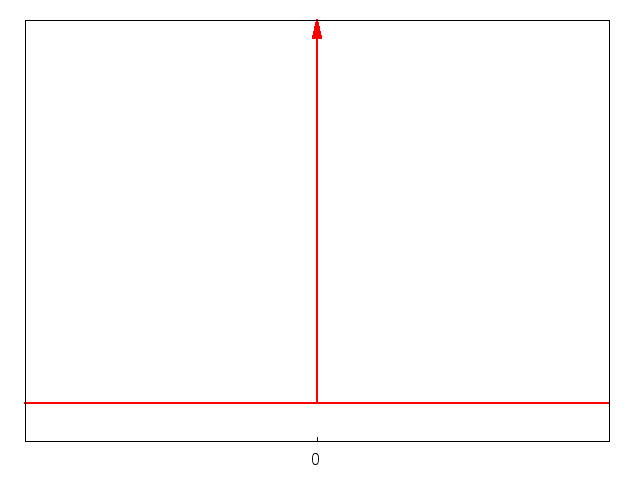
\includegraphics[width=5cm, height=3cm]{plot/funzioni_generalizzate/impulso}
		\end{subfigure}
	\end{figure}
	%
	\linebreak
	L'impulso \'e caratterizzato dal valore della sua area, determinato dal coefficiente della funzione.\\
	%grafico
	\linebreak
	L'impulso torna utile quando bisogna effettuare il \textbf{campionamento} di una funzione, cio\'e determinare il valore della funzione nel punto in cui viene applicato l'impulso.
	\begin{align*}
		f(t)\ \delta(t) &= f(0)\ \delta(t)\\
		f(t)\ \delta(t - T) &= f(T)\ \delta(t - T)   
	\end{align*}
	%
	\section{Doppietto}
	Derivando ulteriormente $\der{}{t}1_{\Delta}(t)$ in un intorno $I(0)$ e in $I(\Delta)$ si ottengo due impulsi unitari: il primo centrato nell'origine, mentre il secondo centrato in $\Delta$ e negativo.\\
	Per $\Delta \longrightarrow 0$ si ottiene:
	\begin{figure}[h!]
		\centering
		\begin{subfigure}{0.5\textwidth}
			\[
			\der{}{t} \delta(t) = \dot{\delta}(t)
			\]
		\end{subfigure}
		\begin{subfigure}{0.4\textwidth}
			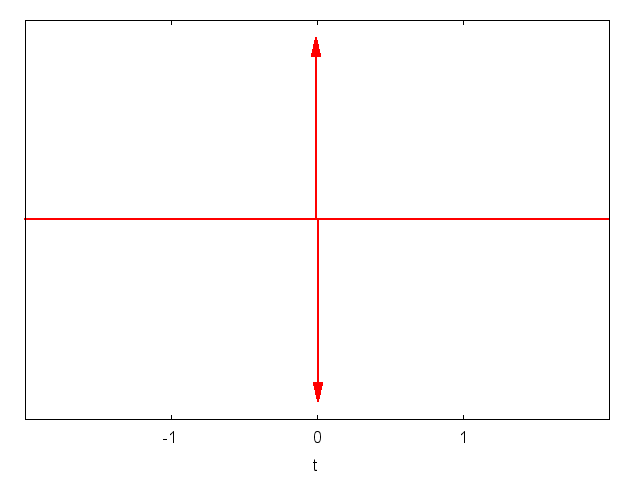
\includegraphics[width=5cm, height=3cm]{plot/funzioni_generalizzate/doppietto}
		\end{subfigure}
	\end{figure}
	%
	\newpage
	\section{Riepilogo}
	$$ 
	par(t) \quad \stackrel[\int_{-\infty}^{t}]{\der{}{t}}{\rightleftharpoons} 
	\quad ramp(t) \quad
	\stackrel[\int_{-\infty}^{t}]{\der{}{t}}{\rightleftharpoons}
	\quad 1(t) \quad
	\stackrel[\int_{-\infty}^{t}]{\der{}{t}}{\rightleftharpoons}
	\quad \delta (t) \quad
	\stackrel[\int_{-\infty}^{t}]{\der{}{t}}{\rightleftharpoons}
	\quad \dot{\delta}(t) \quad
	$$
	%
	\section{Trasformazioni delle funzioni}
	\subsection{Traslazione}
	$$ f(x) = f(x - t) $$
	\begin{itemize}
		\item $ t>0 $: ritardo, la funzione è traslata verso dx di t
		\item $ t<0 $: anticipo, la funzione è traslata verso sx di t 	
	\end{itemize}
	%
	\subsection{Scalamento}
	$$ f(x) = f(x \cdotp t) $$
	\begin{itemize}
		\item $ 0<t<1 $: la funzione si estende di un fattore t
		\item $ t>1 $: la funzione viene compressa di un fattore t  	
	\end{itemize}
	%
	\subsection{Simmetrie}
	\begin{itemize}
		\item $ f(x) = f(-x) $: simmetrica rispetto l'asse delle y
		\item $ f(x) = -f(x) $: simmetrica rispetto l'asse delle x  	
	\end{itemize}
	%
	\section{Altre funzioni di interesse}
	\subsection{Rettangolo}
	%grafico
	$$ R_{t_{1},t_{2}}(t) = 1(t - t_{1}) - 1(t - t_{2}) $$
	%
	\section{Esercizi}
	\subsection{Trasformazione composta di una funzione}
	%
	\subsection{Derivata di una funzione definita a tratti}
	%grafico
	Dividiamo il grafico in sezioni e per ognuna scriviamo la funzione 'finestrata' (cioè moltiplicata per un rettangolo di base pari alla larghezza della sezione):
	$$ f(t) = 2t R_{0,1}(t) + 2 R_{1,3}(t) + (t-4)R_{3,\infty}(t) $$
	Riscriviamo i rettangoli attraverso i gradini:
	\begin{align*}
		f(t) &= 2t\ [1(t) - 1(t-1)] + 2\ [1(t-1) - 1(t-3)] + (t-4)\ [1(t-3) - 0] =\\
		&= 2t\ 1(t) - 2(t-1)\ 1(t-1) + (t-6)\ 1(t-3)
	\end{align*}
	\begin{enumerate}
		\item si riconducono le funzioni a funzioni generalizzate e si deriva:
			\begin{align}
				f(t) &= 2\ ramp(t) & &- ramp(t-1) & &+ (t-3)\ 1(t-3) & - 3\ 1(t-3) \nonumber\\
				\dot{f(t)} &= 2\ 1(t) & &- 2\ 1(t-1) & &+ 1(t-3) & - 3\ \delta(t-3)
				\label{derivata_es2.11.2}
			\end{align}
		\item si usano le derivate del prodotto:
		$$ \dot{f(t)} = (2\ 1(t) + 2t\ \delta(t)) - 2\ 1(t-1) - 2(t-1)\ \delta(t-1) + 1(t-3) + (t-6)\ \delta(t-3) $$
		Attraverso il campionamento si ha che:
		\begin{itemize}
			\item $ t\ \delta(t) = 0 $: campionamento in zero della retta passante per l'origine
			\item $ (t-1)\ \delta(t-1) = 0$: analogo al punto precedente
			\item $ (t-6)\ \delta(t-3) = - 3\ \delta(t-3) $: la retta $ y=t-6 $ calcolata in $ t=3 $ vale -3. 
		\end{itemize}
		Dopo queste semplificazioni si ottiene l'espressione \ref{derivata_es2.11.2}.
	\end{enumerate}
\end{document}